\documentclass[12pt,landscape]{article}
\usepackage[]{media9}

\begin{document}

% \includemedia[activate=pageopen, width=1.0\textwidth, addresource=./Videos/myVideoH.mp4, flashvars={source=./Videos/myVideoH.mp4}]{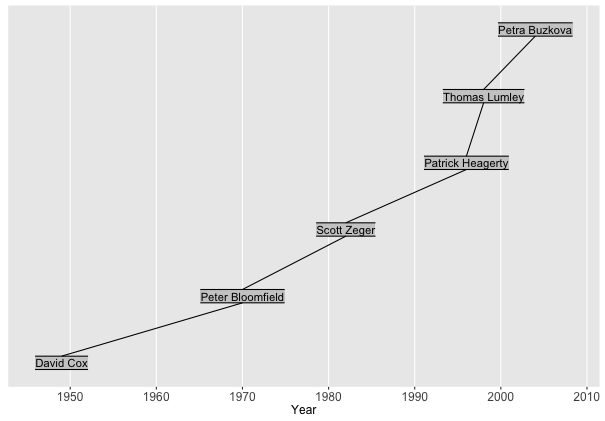
\includegraphics{./pathCB.png}}{VPlayer.swf}

%\includemedia[width=1.0\textwidth, addresource=./Videos/myVideoH.mp4, flashvars={source=./Videos/myVideoH.mp4, &autoPlay=true}]{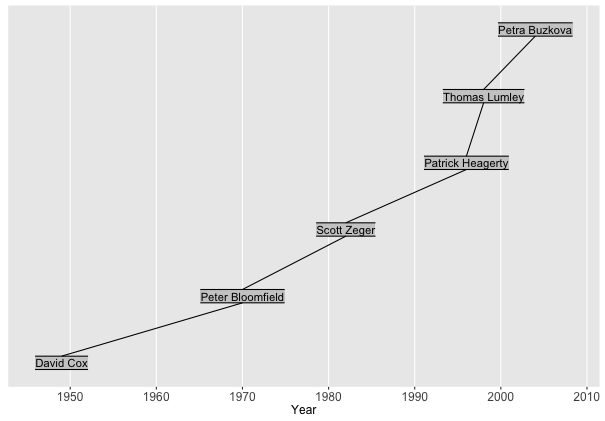
\includegraphics{./pathCB.png}}{VPlayer.swf}

%\includemedia[width=1.0\textwidth, addresource=./Videos/myVideoH.mp4, flashvars={&autoPlay=true, source=./Videos/myVideoH.mp4}]{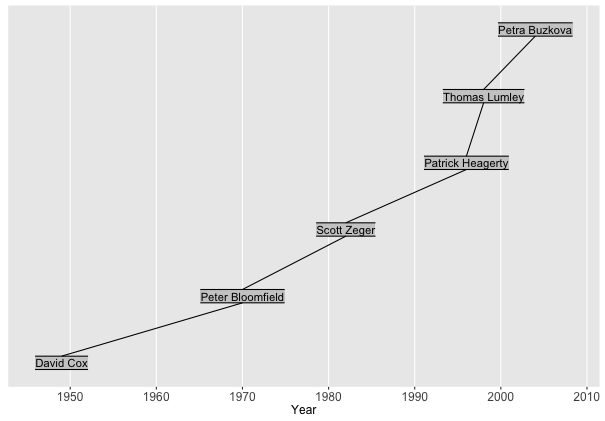
\includegraphics{./pathCB.png}}{VPlayer.swf}

%\includemedia[activate=pageopen, width=1.0\textwidth, addresource=./Videos/myVideoH.mp4, flashvars={&autoPlay=true, source=./Videos/myVideoH.mp4}]{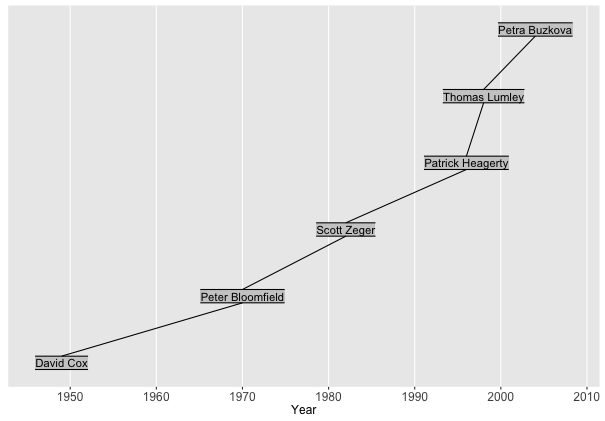
\includegraphics{./pathCB.png}}{VPlayer.swf}

%\includemedia[activate=pageopen, width=1.0\textwidth, addresource=./Videos/myVideoH.mp4, flashvars={source=./Videos/myVideoH.mp4, &autoPlay=true}]{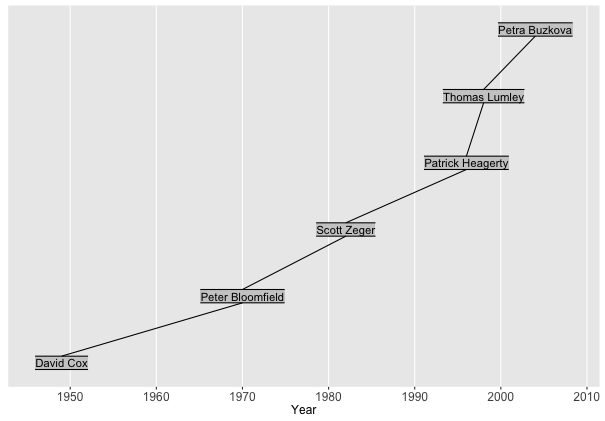
\includegraphics{./pathCB.png}}{VPlayer.swf}

%\includemedia[width=1.0\textwidth, addresource=./Videos/test2.mov, activate=onclick, deactivate=onclick, flashvars={source=./Videos/test2.mov}]{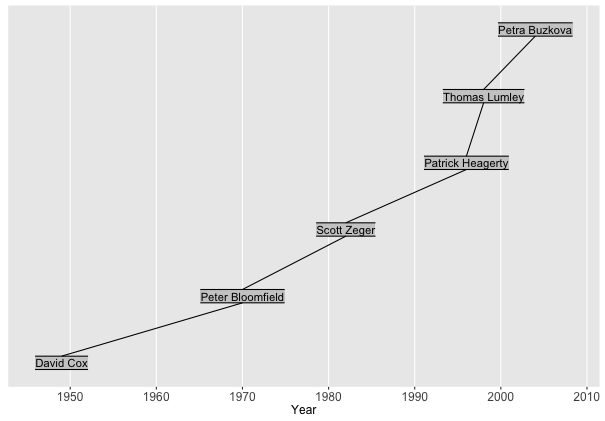
\includegraphics{./pathCB.png}}{VPlayer.swf} % works

%\includemedia[width=1.0\linewidth, addresource=./Videos/test2.mov, activate=pageopen, transparent, flashvars={source=./Videos/test2.mov}]{VPlayer.swf} % works

\includemedia[
  label=myLab,
  width=1.3\linewidth,
  height=0.9\linewidth,
  addresource= ./Videos/test2.mov,
  transparent,
  activate=pageopen,
  passcontext,
  flashvars={
   source=./Videos/test2.mov     % same path as in addresource!
   &loop=true % preserve aspect ratio
  }
]{}{VPlayer.swf}

\mediabutton[
mediacommand=myLab:playPause,
overface=\color{blue}{\fbox{\strut Play/Pause}},
downface=\color{red}{\fbox{\strut Play/Pause}}
]{\fbox{\strut Play/Pause}}
%\mediabutton[
%mediacommand=myLab:setSource [(./Videos/test2.mov)]
%]{\fbox{\strut ./Videos/test2.mov}}


\end{document}
